%%=============================================================================
%% Voorbereiding op het onderzoek
%%=============================================================================

\chapter{Opzet van het onderzoek}
\label{ch:voorbereidingonderzoek}

Voor er aan de slag kan gegaan worden met het onderzoek, moet er een data warehouse opgesteld worden zowel via de Data Vault methodologie als de methodologie voor het dimensioneel modelleren. In dit hoofdstuk wordt de opbouw van het experiment uitgebreid uitgeschreven. Bovendien wordt er ook een overzicht gegeven over de rapporteringsnood voor DHL Pharma Logistics, wat de betekenissen zijn van de gebruikte data in dit onderzoek en hoe een remote connectie moet opgezet worden voor SAP HANA.

\section{Rapporteringsnood DHL Pharma Logistics}
\label{ch:rapporteringsnood}
In deze sectie wordt beschreven wat de rapporteringsnood is voor DHL Pharma Logistics. Er wordt duidelijk beschreven wat de KPI is en deze wordt onderworpen het SMART-principe. 

\subsection{Context}
DHL Pharma Logistics is een divisie van de logistieke grootmacht DHL Supply Chain. PHL Pharma Logistics is verantwoordelijk van de opslag en het bewaren van allerlei medische producten. Bij het stockeren van medische producten moet er met allerlei zaken rekening gehouden worden: temperatuur, houdbaarheid, ... De verantwoordelijkheid van DHL Pharma Logistics ligt bij de opslag en niet bij het vervoeren van deze middelen. DHL Pharma Logistics ontvangt de goederen van labo's (ontwikkelaars van de medicatie) en houden deze goederen bij tot deze moeten verzonden worden naar de klant (ziekenhuizen, apothekers, ...).

\subsection{Dock-to-Stock proces}
De verantwoordelijkheid van DHL Pharma Logistics is om de toegekomen goederen van een pharmaceutische klant te stockeren op de juiste plaats in een vooraf bepaalde tijdspanne. Deze periode wordt opgenomen in een Service Level Agreement (SLA). Het berekenen van deze KPI kan op verschillende niveau's: levering, per pallet of per unit. Bij DHL Pharma Logistics is het gebruikelijk dat goederen moeten worden gestockeerd binnen de 24 uur. Deze KPI wordt dan berekend op pallet-niveau, al zijn er enkele uitzonderingen.

\subsubsection{Dock-to-Stock onderworpen aan het SMART-principe}
Goederen die toekomen aan het magazijn moeten binnen de 24 uur gestockeerd worden op de juiste plaats. In dit interval, moeten alle controles uitgevoerd zijn. Dit is een afspraak die vast gelegd is in de Service Level Agreement met de Labo's.

\begin{itemize}
	\item \textbf{Specifiek: } De KPI is duidelijk geformuleerd.
	\item \textbf{Meetbaar: } Het doel is bereikt wanneer de goederen tijdig zijn gestockeerd.
	\item \textbf{Acceptabel:} De KPI is bepaald in een overeenkomst, dus is deze acceptabel.
	\item \textbf{Realistisch: } Het stockeren van de goederen binnen de 24 uur is realistisch.
	\item \textbf{Tijdsgebonden: } Er wordt een duidelijk interval aangegeven (binnen de 24 uur).
\end{itemize} 

\subsection{De formule voor het berekenen van de KPI}
Een pallet is tijdig gestockeerd wanneer:
\begin{equation*}
\text{Tijdstip van stockage pallet} - \text{Tijdstip van aankomst pallet} < \text{24 uur}
\end{equation*}

\subsection{Hoe moet deze KPI bekeken kunnen worden?}
Deze opgestelde KPI is niet alleen belangrijk voor het cliënteel om na te gaan of de goederen wel tijdig gestockeerd zijn, maar ook voor DHL Pharma Logistics om de juiste analyse te kunnen maken wanneer het fout loopt. Zo kunnen ze opsporen waar er een probleem zit in hun proces en daar de juiste oplossing voor vinden. Hebben ze te weinig personeel voor het verwerken van de orders? Zijn er veel defecten in hun rollend materieel? Hebben ze te veel leveringen geaccepteerd op een te korte termijn? Dit zijn nog maar enkele vragen die kunnen beantwoord worden wanneer een data warehouse is opgesteld voor deze specifieke KPI.

\subsection{Benodigde data}
De data die nodig is voor het uitwerken van de KPI:
\begin{itemize}
	\item Een palletnummer en een levernummer
	\item Tijdstip van levering en stockering.
	\item Klantengegevens
\end{itemize} 

Alle overige data zijn aanvullingen. Deze kunnen dan gebruikt worden om diepere analyses uit te voeren.

\section{Betekenis van de brondata}
\label{sec:betekenisdata}
Vooraleer van start gegaan wordt met het onderzoek, volgt in deze sectie een overzicht (tabel \ref{tab:betekenisdata}) van wat de betekenissen zijn van de gebruikte data. Zo kan de data goed geïnterpreteerd worden. De data die gebruikt wordt is gegenereerde data, en is niet afkomstig uit een bronsysteem van DHL Pharma Logistics. Merk op: de naamgeving van bepaalde data is aangepast (in samenspraak met de business) zodat deze data makkelijker te begrijpen is door de business. Een primary key wordt aangeduid door PK, een foreign key door FK.

\subsection{Overzicht betekenissen}
\begin{center}
	\renewcommand{\arraystretch}{2}%
	\begin{longtable}{  l  l  p{6cm} }
		\textbf{Kolomnaam} & \textbf{Afkomst} & \textbf{Betekenis} \\ \hline
		LABO\_ENTITY\_ID (PK) & Customer\_entities.csv & Een uniek identificatie nummer voor een labo entiteit. 
		Een labo entiteit is een vestiging van een bepaald bedrijf.  \\ \hline
		LABO\_ENTITY\_NAME & Customer\_entities.csv & De vestigingsnaam van de entiteit.  \\ \hline
		LABO\_GROUP\_ID (FK) & Customer\_entities.csv & Identificatienummer van de overkoepelende groep.  \\ \hline
		LABO\_GROUP\_ID (PK) & Customer\_groups.csv & Identificatienummer van de groep.
		Een groep bestaat uit meerdere entiteiten.  \\ \hline
		LABO\_GROUP\_NAAM & Customer\_groups.csv & De naam voor de groep.  \\ \hline
		STAFF\_ID (PK) & Staff.csv & Personeelsnummer van een werknemer.  \\ \hline
		STAFF\_NAME & Staff.csv & De naam van een werknemer.  \\ \hline
		WAREHOUSE\_ID (FK) & Staff.csv & Het warenhuis waar de werknemer actief is.  \\ \hline
		WAREHOUSE\_ID (PK) & Warehouses.csv & Het identificatienummer voor een bepaalde warenhuis.  \\ \hline
		WAREHOUSE\_NAME & Warehouses.csv & De gemeente/stad van het warenhuis (tevens ook de naam).  \\ \hline
		PRODUCT\_ID (PK) & Products.csv & Het artikelnummer. Dit is een uniek nummer.  \\ \hline
		PRODUCT\_DESCRIPTION & Products.csv & Naam/beschrijving van een bepaald product.  \\ \hline
		LABO\_ENTITY\_ID (FK) & Products.csv & Het identificatienummer van de labo entiteit waarvan het product afkomstig is.  \\ \hline
		STATUS\_ID (PK) & Dock\_to\_stock\_status.csv & Identificatienummer van een bepaalde status. 
		Een status wordt gegeven aan een pallet wanneer deze gestockeerd wordt. Ofwel is deze op tijd gestockeerd,
		ofwel is er een bepaalde reden waarom dit niet op tijd kon gestockeerd worden (bijvoorbeeld een te druk moment).  \\ \hline
		STATUS\_DESCRIPTION & Dock\_to\_stock\_status.csv & Beschrijving/uitleg over de status.  \\ \hline
		LEVERAGE\_ID (PK) & Deliveries.csv & Een nummer dat toegekend wordt aan een bepaalde levering.
		Vaak ook een referentienummer dat de klant (labo entiteit) ziet op de factuur. \\ \hline
		PALLET\_ID & Deliveries.csv & Het identificatienummer van een pallet.
		Een levering kan uit meerdere palletten bestaan. \\ \hline
		STAFF\_ID (FK) & Deliveries.csv & Een personeelsnummer. 
		Dit personeelslid was verantwoordelijk voor het juist en tijdig (binnen de afgesproken periode met de labo entiteit) stockeren van een pallet. \\ \hline
		PRODUCT\_ID (FK) & Deliveries.csv & Het identificatienummer van het product dat gestockeerd werd.
		Er wordt enkel 1 productsoort op een pallet gestockeerd. \\ \hline
		PRODUCT\_QUANTITY & Deliveries.csv & De hoeveelheid producten aanwezig op een pallet.
		De hoeveelheid wordt weergegeven per unit. \\ \hline
		DOCK\_TIME & Deliveries.csv & Het tijdstip waarop de pallet toekomt in het magazijn. \\ \hline
		STOCK\_TIME & Deliveries.csv & Het tijdstip waarop de pallet gestockeerd werd op de juiste plaats. \\ \hline
		STATUS\_ID (FK) & Deliveries.csv & Identificatienummer voor de status. Indien deze tijdig werd gestockeerd, dan werd geen status toegekend. \\
		\caption{Betekenis van de gebruikte data in dit experiment.}
		\label{tab:betekenisdata}
	\end{longtable}
\end{center}

\section{Gebruikte technologieën in dit experiment}
De benodigdheden voor het nabootsen van dit experiment zijn:

\begin{itemize}
	\item \textbf{SAP HANA technologie:} deze databank draait op een Linux distributie (Debian) in een Azure omgeving.\footnote[1]{De SAP HANA server moet bereikbaar zijn over het internet.}
	\item \textbf{Databron:} Als databron worden csv-bestanden gebruikt die aangeleverd worden door een Windows server (versie 2016) die draait in een Azure omgeving.\footnote[2]{De Windows server moet bereikbaar zijn over het internet.}
	\item \textbf{Data Provisioning Agent:} De DP Agent wordt gebruikt om een bron te verbinden met SAP HANA.
	\item \textbf{SDI:} Een ETL-tool die aangeleverd wordt door SAP en die geïntegreerd is binnen SAP HANA.
\end{itemize}

In dit onderzoek worden voornamelijk SAP producten gebruikt. De reden hiervoor is omdat er binnen DHL Pharma Logistics ook voornamelijk gewerkt wordt met SAP producten.

\section{Overzicht van de connectie tussen SAP HANA en de host}
\begin{figure}[h]
	\centering
	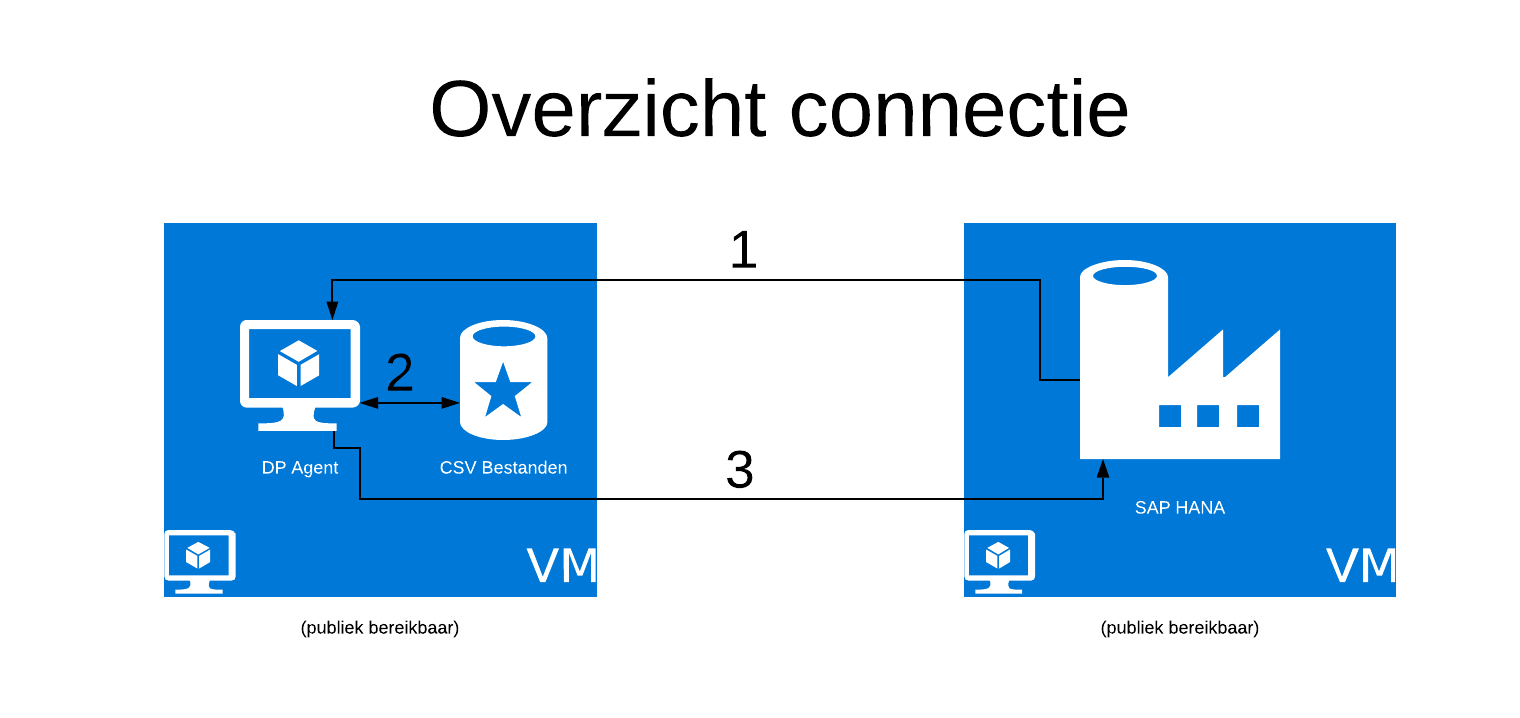
\includegraphics[scale=0.5]{../images/AzureConnectieBP.png}
	\caption{Voorstelling netwerk (gemaakt via Lucidchart.com).}
	\label{fig:azureconn}
\end{figure}

In figuur \ref{fig:azureconn} zijn beide virtuele machines bereikbaar op het internet zodat de connectie tussen beiden mogelijk is. Op de virtuele machine waar de DP Agent op draait staat bovendien ook poort 5050 open en maakt gebruik van het TCP protocol. Dit protocol zorgt ervoor dat elk datapakket arriveert op zijn bestemming in tegenstelling tot UDP. Wanneer snelheid belangrijk (Skype, streaming, ..) is, kies je voor UDP. Dit protocol zal nooit gebruikt worden bij deze soort connectie.

Hieronder een overzicht over hoe de verbinding in zijn werk gaat:

\begin{enumerate}
	\item SAP HANA stuurt een request voor data naar de DP Agent die geïnstalleerd staat op de host.
	\item De host haalt de benodigde data op via een adapter, in dit geval haalt hij de CSV-files die nodig zijn op uit een lokale betandslocatie.
	\item De DP Agent zendt de data door naar SAP HANA.
\end{enumerate}

\section{Opzetten van een remote source}
Wanneer er een verbinding moet opgezet worden naar SAP HANA, moet een Data Provisioning Agent (zie figuur \ref{fig:dpa}) geïnstalleerd worden. Deze wordt geïnstalleerd op de host die een verbinding moet maken met SAP HANA. Nadat deze geïnstalleerd is, moet deze ook nog geconfigureerd worden. Volgende zaken moeten zeker in orde gebracht worden voor een connectie kan plaats vinden: 
\interfootnotelinepenalty=10000
\begin{itemize}
	\item Connection: de agent moet geconnecteerd en ingelogd zijn op het SAP HANA systeem.
	\item Registered: de agent moet geregistreerd zijn bij SAP HANA.
	\item Adapter: de juiste adapter (in dit onderzoek: FileAdapter) moet geregistreerd zijn bij SAP HANA\footnote[1]{Een bronsysteem kan meerdere databronnen bevatten (bijvoorbeeld zowel CSV-bestanden als een MySQL databank). Daarom is het noodzakelijk de juiste adapter te registreren bij SAP HANA.}. Bovendien moet de adapter ook correct geconfigureerd zijn (juiste parameters).
\end{itemize} 

\begin{figure}[h]
	\centering
	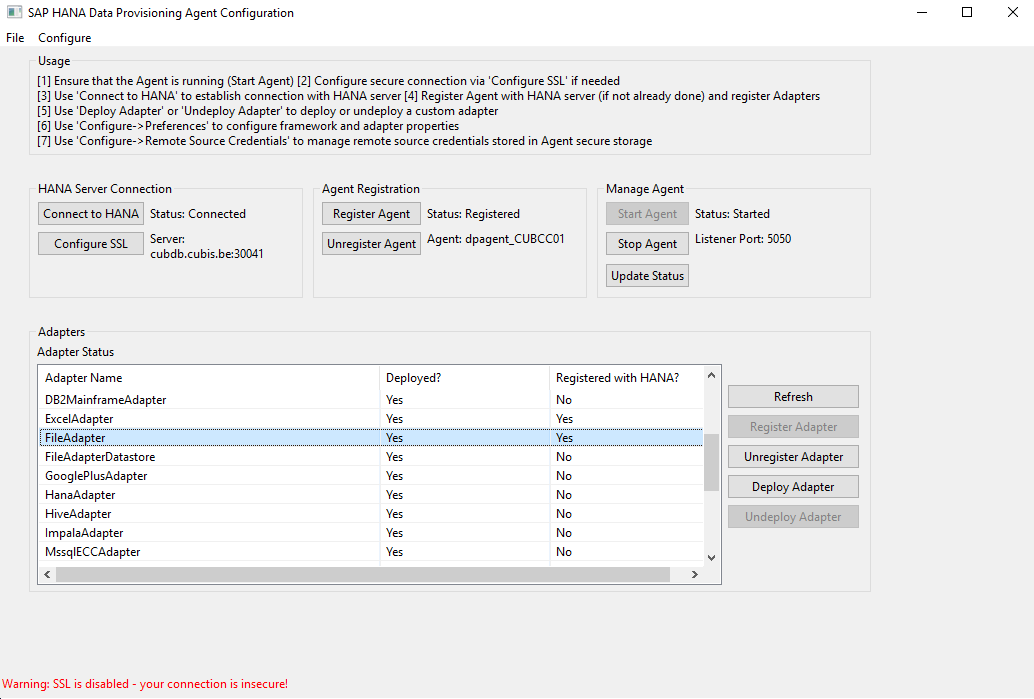
\includegraphics[scale=0.5]{../images/DPAgent.png}
	\caption{DP Agent verbonden met SAP HANA.}
	\label{fig:dpa}
\end{figure}

Wanneer alles correct geconfigureerd is, kan er nu vanuit SAP HANA een remote connectie (zie figuur \ref{fig:remoteconn}) gemaakt worden naar de host en kan de benodigde informatie opgevraagd worden.

\begin{figure}[h]
	\centering
	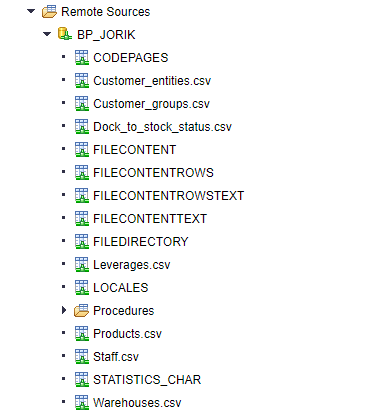
\includegraphics[scale=0.5]{../images/remoteconn.png}
	\caption{Een remote connectie opgezet naar de host vanuit SAP HANA.}
	\label{fig:remoteconn}
\end{figure}

\section{Data Vault: data warehousing}
\label{ch:dvmodel}
In deze sectie wordt een data warehouse opgebouwd aan de hand van Data Vault. Elke laag van de architectuur (en de bijhorende ETL) komt aan bod. Op het einde van dit hoofdstuk moet er via een rapporteringsomgeving kunnen verbonden worden met een ontworpen data mart, gebaseerd op een data warehouse ontworpen met de Data Vault methodologie, om de benodigde gegevens te kunnen opvragen.

\subsection{Overzicht datamodel}
\begin{figure}[h]
	\centering
	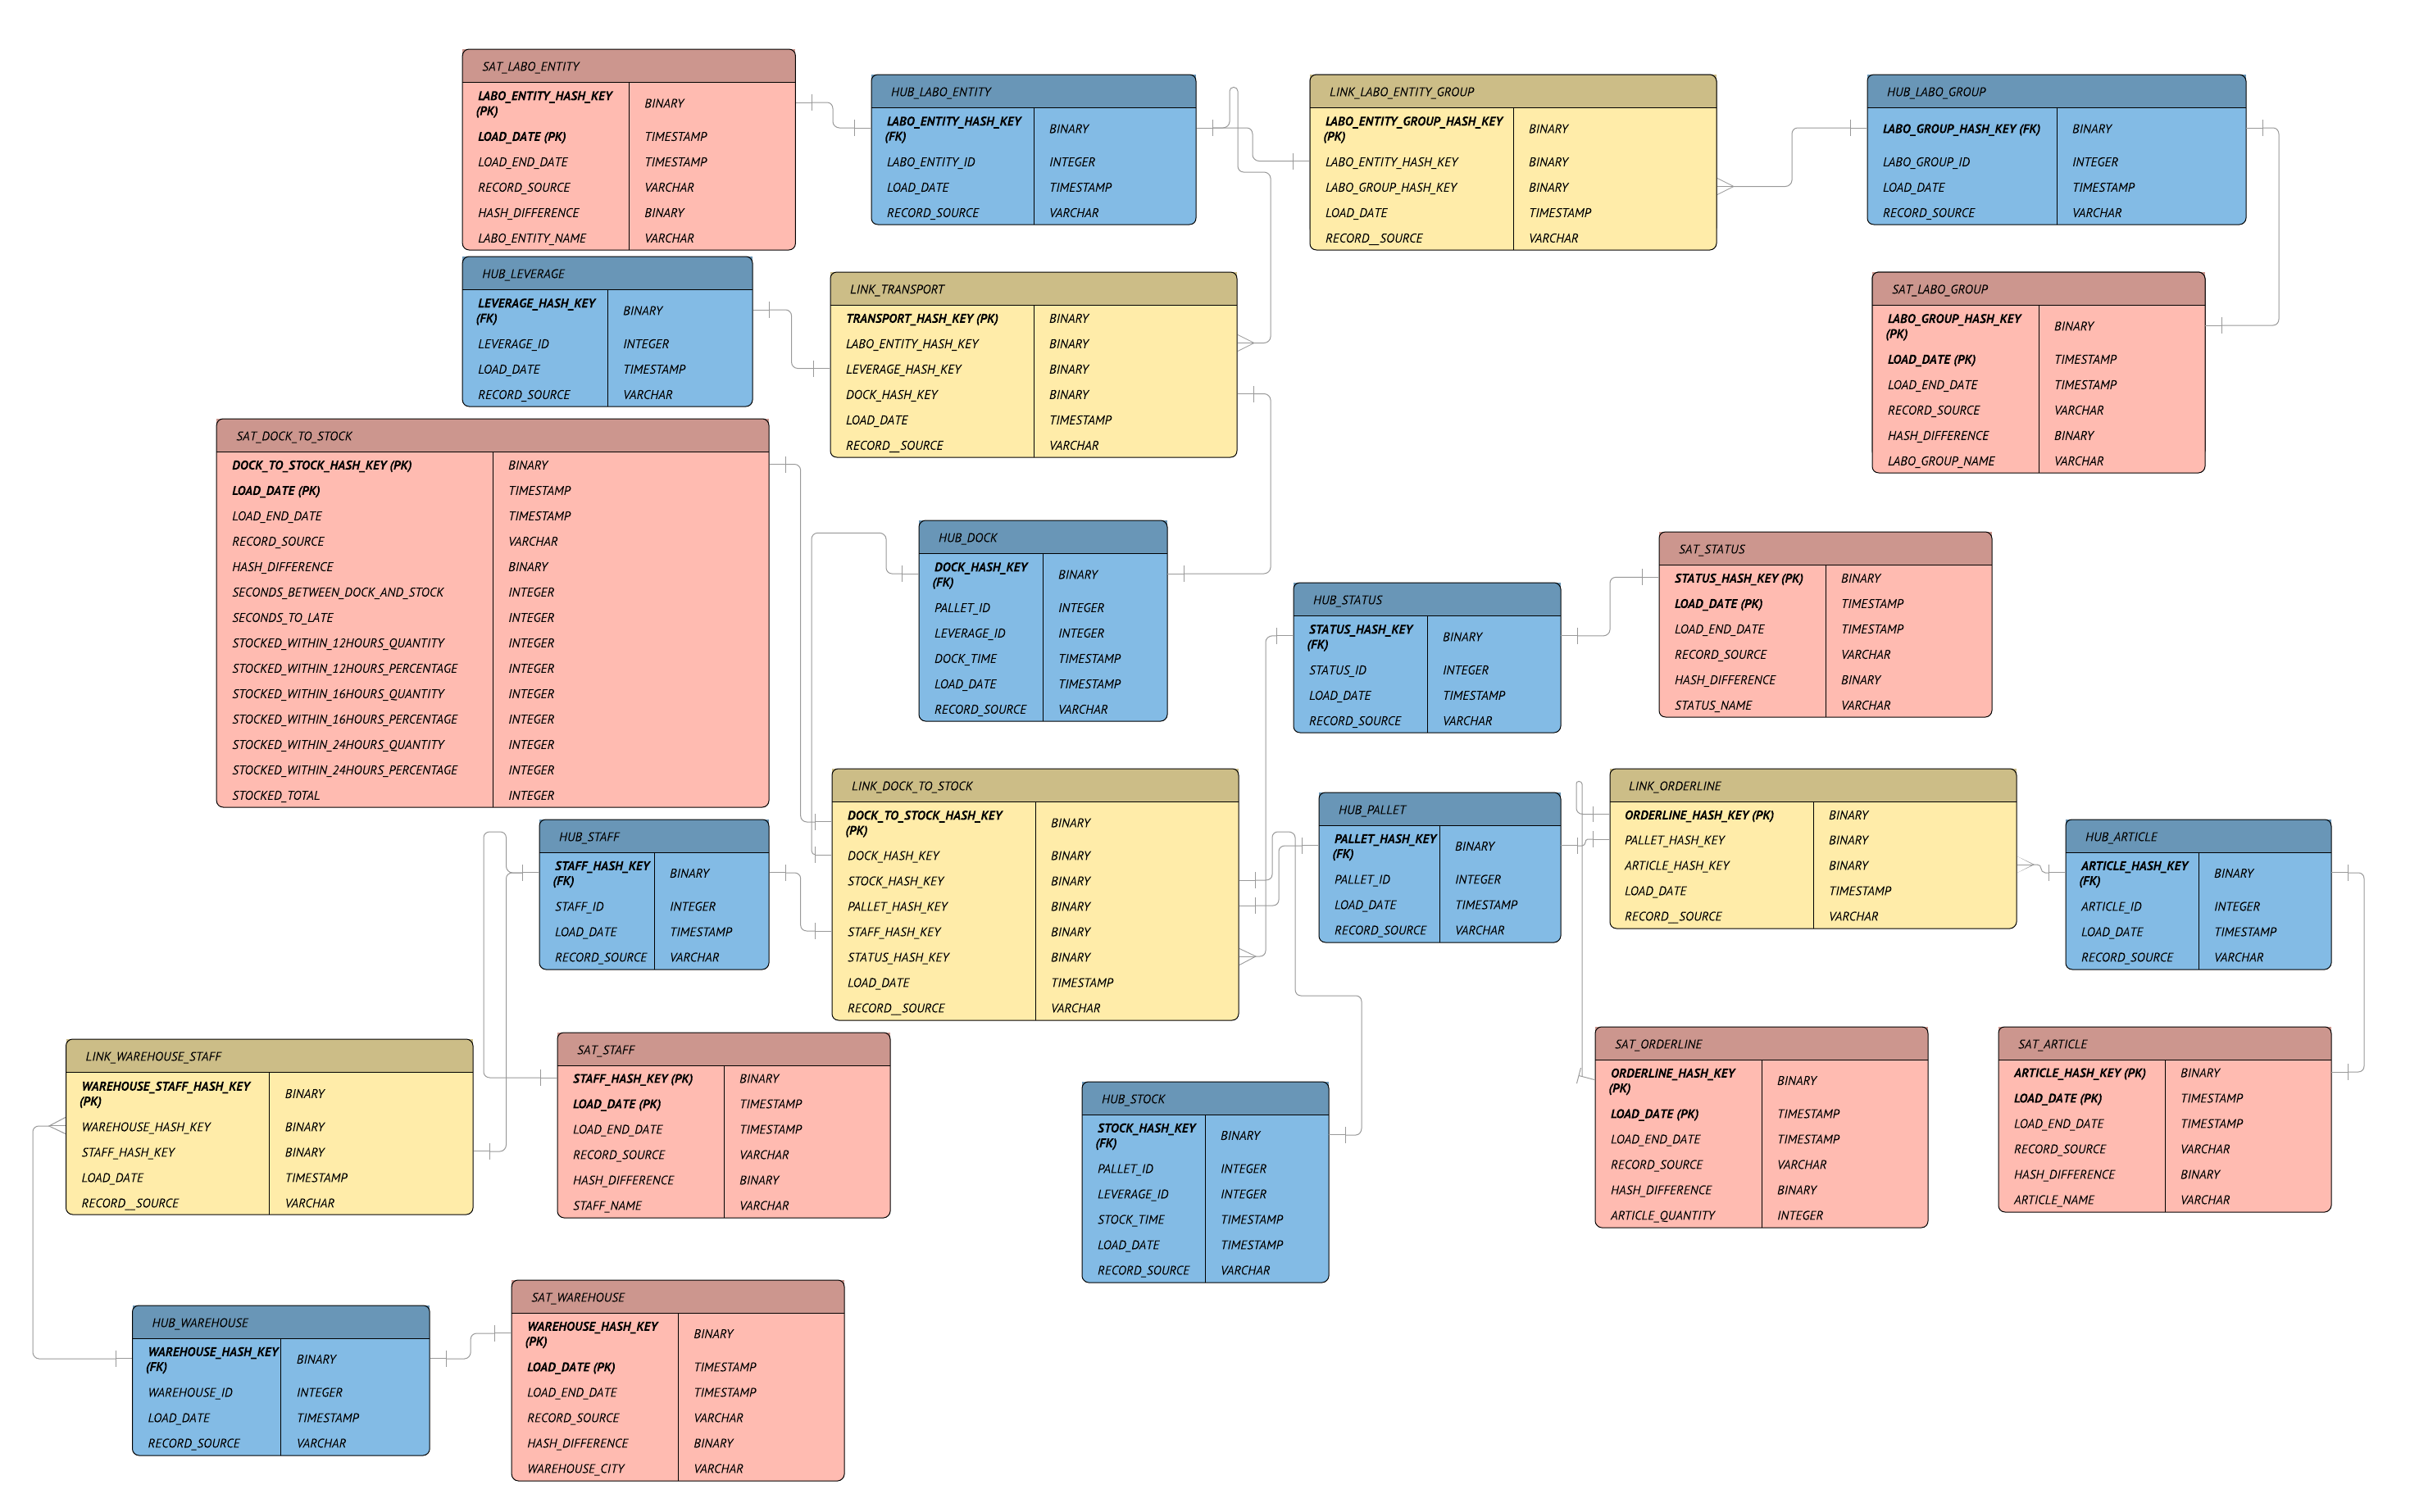
\includegraphics[scale=0.34]{../images/DataVaultModel.png}
	\caption{Voorstelling van het Data Vault model (gemaakt via Lucidchart.com).}
	\label{fig:dvm}
\end{figure}

Het model in figuur \ref{fig:dvm} is opgebouwd uit drie soorten tabellen: de rode entiteiten worden voorgesteld als sattelites, de blauwe entiteiten als hubs en de gele entiteiten vormen de links tussen de verschillende hubs. In de SAT\_DOCK\_TO\_STOCK worden de berekeningen opgeslagen die nodig zijn voor het berekenen van de KPI. Hash keys worden opgeslagen onder het type ''binary''.

\subsection{Staging area}
\label{sec:stagareadv}
In de staging area worden alle gegevens in de originele vorm ingeladen. Dit betekent dat hierop nog geen manipulaties mogen gebeuren. In dit onderzoek wordt de data ingeladen via een virtuele tabel, afkomstig van een remote source (zie figuur \ref{fig:stag}).

\begin{figure}[h]
	\centering
	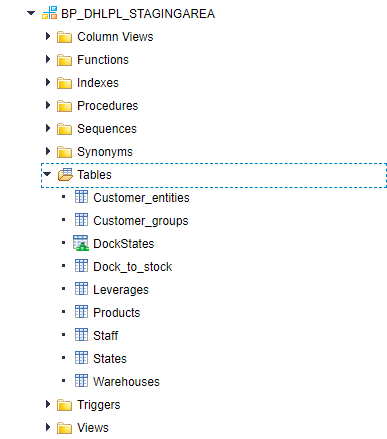
\includegraphics[scale=0.45]{../images/DV_staging.png}
	\caption{Toevoegen van virtuele tabellen aan de staging area (SAP HANA).}
	\label{fig:stag}
\end{figure}

Eens alle virtuele tabellen toegevoegd zijn in de staging area, dan is het modelleren van de eerste laag afgewerkt en kan er overgegaan worden naar het modelleren van de raw Data Vault.

\subsection{Opbouw raw Data Vault}
In de raw Data Vault wordt de source data omgevormd naar de Data Vault methodologie. Hierbij wordt nog geen extra business logica en/of berekeningen toegevoegd. Concreet voor dit data model zullen de gegevens getransformeerd worden en doorgeladen worden naar alle tabellen, behalve de tabel SAT\_DOCK\_TO\_STOCK (business logica). De data bij de tabel HUB\_DOCK\_TO\_STOCK kan wel al ingeladen worden, aangezien deze geen business logica bevat (een hub of link bevat nooit business logica).

\subsubsection{Inladen van data bij een sattelite}
Het inladen \& transformeren van de data bij alle sattelites binnen de raw Data Vault gebeurt gelijkaardig. In dit voorbeeld wordt het ETL-proces weergegeven van SAT\_ORDERLINE en uitgelegd welke stappen ondernomen moeten worden om de data juist in te laden.
\begin{figure}[h]
	\centering
	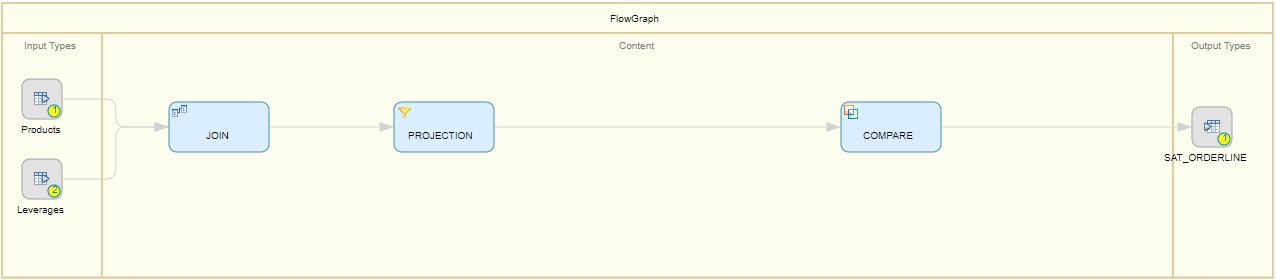
\includegraphics[scale=0.45]{../images/DV_FG_sattelite.png}
	\caption{Een voorbeeld van een ETL proces in SAP HANA bij een sattelite (SAP SDI).}
	\label{fig:etlsat}
\end{figure}

In de eerste stap van dit proces worden verschillende bronnen (afkomstig uit de staging area) samengevoegd naar 1 dataset op basis van een gemeenschappelijk attribuut. Alle onnodige data wordt niet meegenomen naar de volgende stap. Deze stap kan ook overgeslagen worden indien de benodigde data afkomstig is uit één bron.

Vervolgens wordt de data getransformeerd naar het juiste formaat (naar het formaat van de destination tabel). Bij de tabel SAT\_ORDERLINE worden volgende manipulaties uitgevoerd:

\begin{itemize}
	\item \textbf{ORDERLINE\_HASH\_KEY (PK):} Een gehashte sleutel van volgende componenten: ''PRODUCT\_ID'' (tabel Products), ''PALLET\_ID'' (tabel Leverages) en de naam van het bronsysteem (in dit geval: ''DATAFILES'').
	\item \textbf{LOAD\_DATE (PK):} Datum/tijdstip wanneer de record geëxtraheerd werd uit de bron.
	\item \textbf{LOAD\_END\_DATE:} Tijdstip tot wanneer de data actueel was, indien deze nog steeds actueel is, krijgt deze de waarde ''9999/12/31 23:59:59'' (belangrijk voor de historiek).
	\item \textbf{RECORD\_SOURCE:} De naam van het bronsysteem waarvan de data afkomstig is (''DATAFILES'' in dit geval).
	\item \textbf{HASH\_DIFFERENCE:} Alle data afkomstig in de entiteit die wordt opgenomen in het Data Vault model, wordt gehasht naar 1 sleutel. In dit geval wordt enkel ''ARTICLE\_QUANTITY'' versleuteld. 
	\item \textbf{ARTICLE\_QUANTITY:} Het attribuut ''PRODUCT\_QUANTITY'' wordt overgenomen van de brondata.
\end{itemize} 

Nadat de transformaties gebeurd zijn, vergelijken we de nieuwe data met de data die in de destination table zit. Indien de data een nieuwere versies bevat, dan zal deze toegevoegd worden en de ''LOAD\_END\_DATE'' van de oude entiteit gewijzigd worden naar het tijdstip van extractie van de nieuwe entiteit.

\subsubsection{Inladen van data bij een hub}
In elke hub worden de entiteiten bijgehouden die gebruikt zullen worden, en die het meest geschikt zijn voor de rapportering. Deze kunnen ook opgebouwd worden aan de hand van het principe van de "golden record", waarbij de data van verschillende bronnen samengevoegd worden tot één record, om zo een compleet en correct mogelijke record te verkrijgen. In dit onderzoek is dit niet het geval, aangezien er gewerkt wordt met één bron. 

\begin{figure}[h]
	\centering
	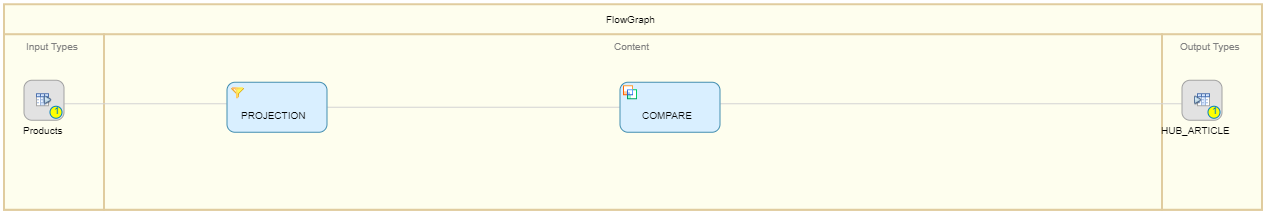
\includegraphics[scale=0.45]{../images/DV_FG_hub.png}
	\caption{Een voorbeeld van een ETL proces in SAP HANA bij een hub (SAP SDI).}
	\label{fig:etlhub}
\end{figure}

Bij de projectie worden volgend transformaties toegepast:

\begin{itemize}
	\item \textbf{ARTICLE\_HASH\_KEY (PK):} Een gehashte sleutel van volgende componenten: ''PRODUCT\_ID'' (tabel Products) en de naam van het bronsysteem (in dit geval: ''DATAFILES'').
	\item \textbf{ARTICLE\_ID:} De business key van de entiteit ''Article'' wordt overgenomen van de brondata.
	\item \textbf{LOAD\_DATE:} Datum/tijdstip wanneer de record geëxtraheerd werd uit de bron.
	\item \textbf{RECORD\_SOURCE:} De naam van het bronsysteem waarvan de data afkomstig is (''DATAFILES'' in dit geval).
\end{itemize}

\subsubsection{Inladen van data bij een link}
Bij het inladen voor de data in de link-entiteiten worden dezelfde stappen doorlopen als bij het inladen van data bij hubs en sattelites. Links stellen de relaties voor tussen de verschillende entiteiten. 

\begin{figure}[h]
	\centering
	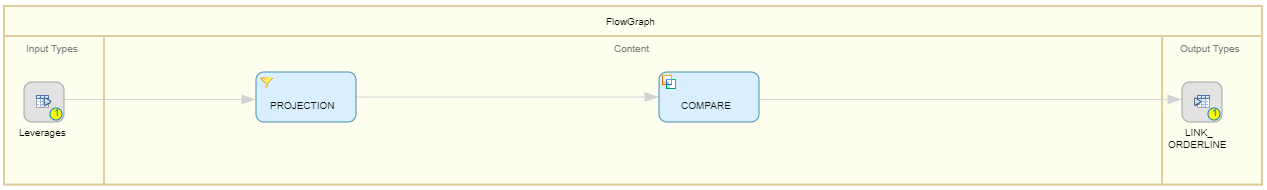
\includegraphics[scale=0.45]{../images/DV_FG_link.png}
	\caption{Een voorbeeld van een ETL proces in SAP HANA bij een link (SAP SDI).}
	\label{fig:etllink}
\end{figure}

\begin{itemize}
	\item \textbf{ORDERLINE\_HASH\_KEY (PK):} Een gehashte sleutel van volgende componenten: ''PRODUCT\_ID'' (tabel Leverages), ''PALLET\_ID'' (tabel Leverages)  en de naam van het bronsysteem (in dit geval: ''DATAFILES'').
	\item \textbf{ARTICLE\_HASH\_KEY:} Een gehashte sleutel van volgende componenten: ''PRODUCT\_ID'' (tabel Leverages).
	\item \textbf{PALLET\_HASH\_KEY:} Een gehashte sleutel van volgende component: ''PALLET\_ID'' (tabel Leverages).
	\item \textbf{LOAD\_DATE:} Datum/tijdstip wanneer de record geëxtraheerd werd uit de bron.
	\item \textbf{RECORD\_SOURCE:} De naam van het bronsysteem waarvan de data afkomstig is (''DATAFILES'' in dit geval).
\end{itemize}

\subsection{Opbouw business vault}
Aangezien de Business vault in dit data schema slechts 1 nieuwe entiteit bevat, vertelt de methodologie van Data Vault dat het niet nodig is om een nieuwe laag hiervoor te ontwerpen (besparen van opslagruimte). De business vault tabellen mogen dan toegevoegd worden aan de raw Data Vault indien dit de complexiteit niet aanzienlijk zou verhogen.

Bij het aanmaken van het ETL proces bij een sattelite binnen de Business vault, worden dezelfde stappen overlopen als bij het aanmaken van een sattelite binnen de raw Data Vault. Bij ''projection'' wordt dan de benodigde business logica en de benodigde berekeningen toegevoegd.

\subsection{Opbouw data mart}
Wanneer alle data getransformeerd en ingeladen is in de Data Vault modellen, moeten deze verbonden worden met elkaar en wordt hiervoor een virtuele view aangemaakt waarop verbonden kan worden vanuit een rapporteringsomgeving (zie figuur \ref{fig:dvdm}).

Een best practice die in dit onderzoek werd toegepast was het samenvoegen van alle hubs, links \& sattelites in één dimensie. Zo wordt een beter overzicht behouden van de opgestelde calculation views en wordt de complexiteit verminderd. Deze dimensie werd dan verbonden met een fact table in een sterschema. 

\begin{figure}[h]
	\centering
	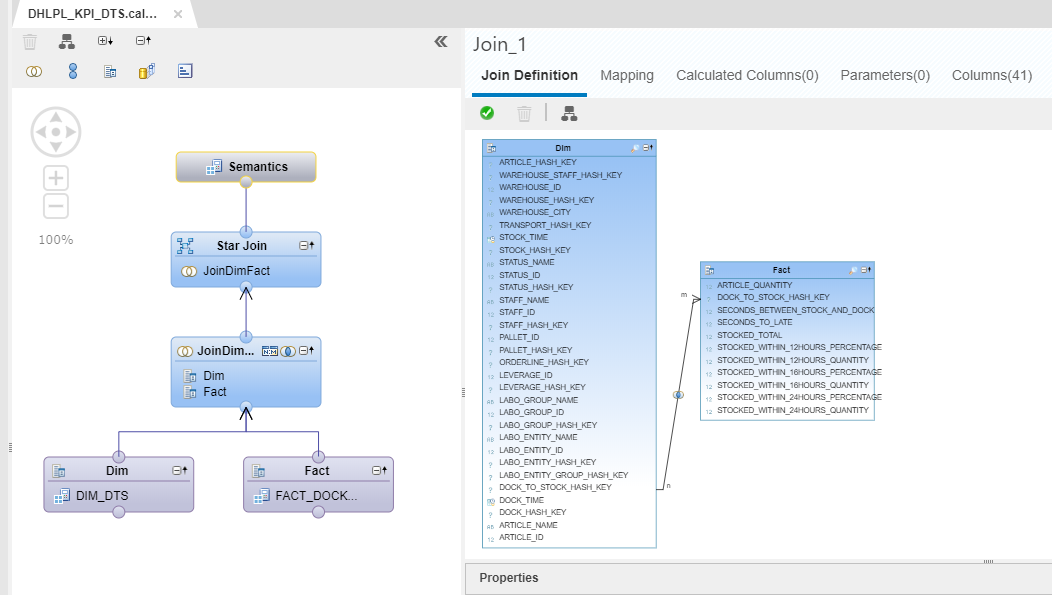
\includegraphics[scale=0.5]{../images/DV_FG_datamart.png}
	\caption{Sterschema opgesteld in SAP voor Data Vault.}
	\label{fig:dvdm}
\end{figure}

\section{Dimensioneel model: data warehousing}
\label{ch:dimmodel}
In dit hoofdstuk wordt een data warehouse opgebouwd aan de hand van het dimensioneel modelleren. Net zoals bij het Data Vault model, moet hier alles geconfigureerd worden zodat een verbinding mogelijk is vanuit een rapporteringsomgeving.

\subsection{Overzicht datamodel}
\begin{figure}[h]
	\centering
	\includegraphics[scale=0.5]{../images/Dimensioneelmodel.png}
	\caption{Voorstelling van het dimensioneel model (gemaakt via Lucidchart.com).}
	\label{fig:dmdm}
\end{figure}

In figuur \ref{fig:dmdm}  worden de dimensions voorgesteld als de blauwe entiteiten. Deze bevatten de beschrijvende data die iets meer vertellen over de ''facts''. De business key wordt gebruikt als attribuut die de relatie legt naar de facts-table (die wordt voorgesteld in het rood). In dit model worden geen gegevens opgeslagen die meer vertellen over de oorsprong van de data, tevens wordt de historiek van de data niet bijgehouden.

\subsection{Staging area}
In de architectuur van Data Vault, is al reeds een staging area toegevoegd die alle informatie ongemanipuleerd bijhoudt. Voor dit onderdeel van het onderzoek zal de laag niet opnieuw worden toegevoegd, maar zal er gebruik gemaakt worden van de eerder toegevoegde laag (zie sectie \ref{sec:stagareadv}).

\subsection{Opbouw data warehouselaag}
In deze sectie wordt de data warehouselaag opgebouwd. In tegenstelling tot Data Vault wordt alle data in deze laag weggeschreven, inclusief de business logica die berekend moet worden. De benodigde data wordt opgehaald uit de staging area.

\subsubsection{Dimensions}
Bij het inladen van de dimensions bij het dimensioneel model, moeten er nooit berekeningen uitgevoerd worden, aangezien deze de beschrijvende data bevatten over de facts. Wel kan de data in dit proces gecleaned en gemanipuleerd worden om een betere structuur te krijgen. 

\begin{figure}[h]
	\centering
	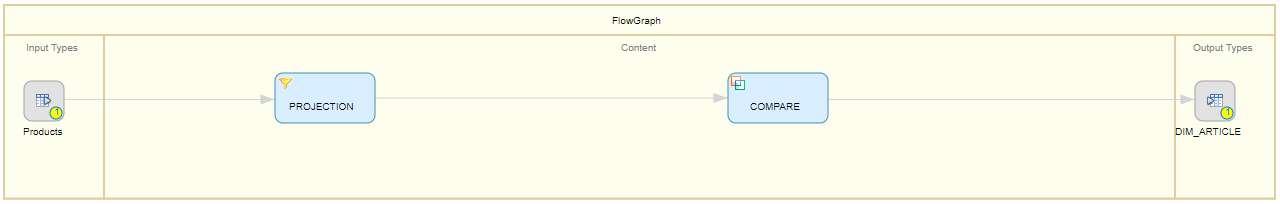
\includegraphics[scale=0.5]{../images/DM_FG_dim.png}
	\caption{Voorstelling van het ETL-proces bij een dimension (SAP SDI).}
	\label{fig:DM_FG_dim}
\end{figure}

In figuur \ref{fig:DM_FG_dim}  wordt het ETL-proces voorgesteld bij het inladen van de data in de tabel DIM\_ARTICLE. Aangezien er enkel data moet ingeladen worden vanuit één enkele tabel, moet er geen JOIN gebeuren. Er kan dus onmiddellijk begonnen worden met het transformeren van de data in PROJECTION. 

\begin{itemize}
	\item \textbf{ARTICLE\_ID (PK):} In dit attribuut wordt PRODUCT\_ID overgenomen van de brondata.
	\item \textbf{ARTICLE\_NAME:} In dit attribuut wordt PRODUCT\_DESCRIPTION overgenomen van de brondata.
\end{itemize} 

In de stap COMPARE wordt vergeleken of de nieuwe record al aanwezig is in de databank. Indien dit niet het geval is, wordt deze toegevoegd, anders wordt de record in de databank met dezelfde key overschreven. Bij het dimensioneel model wordt geen historiek bijgehouden van gegevens.

\subsubsection{Facts}
Bij een fact tabel, wordt de key van elke dimension bijgehouden. Alle sleutels samen vormen een composite key die dan geldt als primary key. Dit zorgt voor een zekere complexiteit bij het opbouwen van het ETL-proces. In dit proces worden ook de berekeningen uitgevoerd die nodig zijn voor het uitrekenen of de KPI wel/niet bereikt is.

\begin{figure}[h]
	\centering
	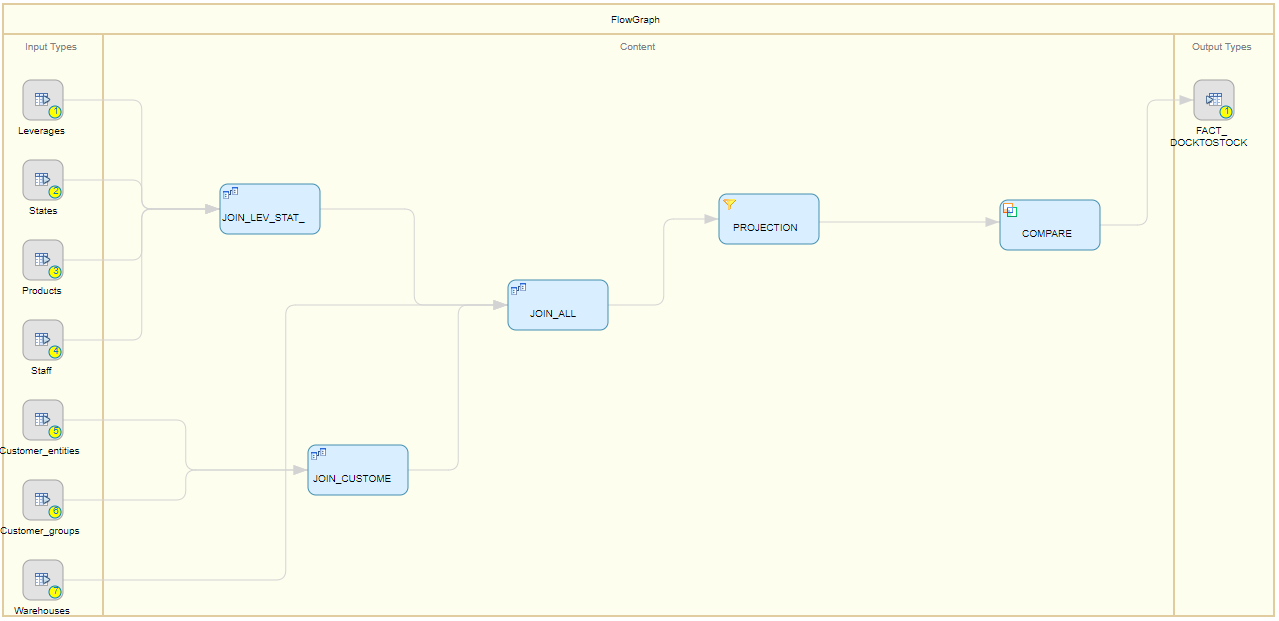
\includegraphics[scale=0.5]{../images/DM_FG_fact.png}
	\caption{Voorstelling van het ETL-proces bij een fact (SAP SDI).}
	\label{fig:DM_FG_fac}
\end{figure}

In de eerste stap van figuur \ref{fig:DM_FG_fac} (JOIN\_LEV\_STAT\_PROD\_STAFF) wordt de data van de tabellen Leverages, States, Products en Staff samengevoegd op basis van de aanwezige attributen in de source tabel Leverages. Alleen de benodigde data wordt meegenomen naar de volgende stap. Bij JOIN\_CUSTOMER wordt tussen de tabellen Customer\_Entities en Customer\_Groups een relatie gelegd. Om uiteindelijk alles samen te voegen tot één geheel, wordt er een finale join (JOIN\_ALL) aangelegd. Hierbij wordt de data van JOIN\_LEV\_STAT\_PROD\_STAFF, JOIN\_CUSTOMER en Warehouses gecombineerd die kan gebruikt worden in de volgende stappen.

Vervolgens wordt de benodigde data berekend. Volgende transformaties worden toegepast:

\begin{itemize}
	\item \textbf{STAFF\_ID (PK):} In dit attribuut wordt STAFF\_ID overgenomen van de brondata.
	\item \textbf{ARTICLE\_ID (PK):} In dit attribuut wordt PRODUCT\_ID overgenomen van de brondata.
	\item \textbf{STATUS\_ID (PK):} In dit attribuut wordt STATUS\_ID overgenomen van de brondata.
	\item \textbf{WAREHOUSE\_ID (PK):} In dit attribuut wordt WAREHOUSE\_ID overgenomen van de brondata.
	\item \textbf{LABO\_ENTITY\_ID (PK):} In dit attribuut wordt LABO\_ENTITY\_ID overgenomen van de brondata.
	\item \textbf{LEVERAGE\_ID (PK):} In dit attribuut wordt LEVERAGE\_ID overgenomen van de brondata.
	\item \textbf{PALLET\_ID (PK):} In dit attribuut wordt PALLET\_ID overgenomen van de brondata.
	\item \textbf{LABO\_GROUP\_ID (PK):} In dit attribuut wordt LABO\_GROUP\_ID overgenomen van de brondata.
	\item \textbf{ARTICLE\_QUANTITY :} In dit attribuut wordt PRODUCT\_QUANTITY overgenomen van de brondata.
	\item \textbf{TOTAL\_STOCKED :} In dit attribuut wordt het getal '1' opgeslagen. Zo kan er na de aggregatie een deling uitgevoerd worden om een bepaald percentage uit te rekenen. Tevens zorgt dit ook voor een duidelijke naam voor de business.
	\item \textbf{SECONDS\_TO\_LATE :} Indien het verschil tussen STOCK\_TIJD en DOCK\_TIJD kleiner is dan 86400 seconden (24u), dan is het resultaat 0. Indien dat verschil groter is dan 86400 seconden, dan wordt het verschil tussen STOCK\_TIJD en DOCK\_TIJD weergegeven.
	\item \textbf{SECONDS\_BETWEEN\_DOCK\_AND\_STOCK :} In dit attribuut wordt het verschil tussen STOCK\_TIJD en DOCK\_TIJD weergegeven.
	\item \textbf{STOCKED\_WITHIN\_12HOURS\_QUANTITY :} Indien de pallet gestockeerd werd binnen de 12 uur tijd, dan is de waarde van dit attribuut 1, anders 0.
	\item \textbf{STOCKED\_WITHIN\_16HOURS\_QUANTITY :} Indien de pallet gestockeerd werd binnen de 16 uur tijd, dan is de waarde van dit attribuut 1, anders 0.
	\item \textbf{STOCKED\_WITHIN\_24HOURS\_QUANTITY :} Indien de pallet gestockeerd werd binnen de 24 uur tijd, dan is de waarde van dit attribuut 1, anders 0.
\end{itemize} 

Nadat alle transformaties en berekeningen zijn toegepast, worden de toegekomen waardes vergeleken met de huidige waardes van de destination table. Er wordt vergeleken op basis van de composite key. Indien de waarde al in de database aanwezig is, wordt deze overschreven, anders wordt deze toegevoegd aan de dataset.

\subsection{Opbouw data mart}
Nadat alle tabellen in het dimensioneel model zijn aangevuld, kan er een data mart aangemaakt worden voor de opgestelde KPI. Dit gebeurt gelijkaardig zoals bij het Data Vault model. Er zal een sterschema aangemaakt worden waarbij alle dimensions verbonden worden (zie figuur \ref{fig:dmdmart}) met de fact tabel. Hierop kan dan verbonden worden vanuit een rapporteringsomgeving. 

\begin{figure}[h]
	\centering
	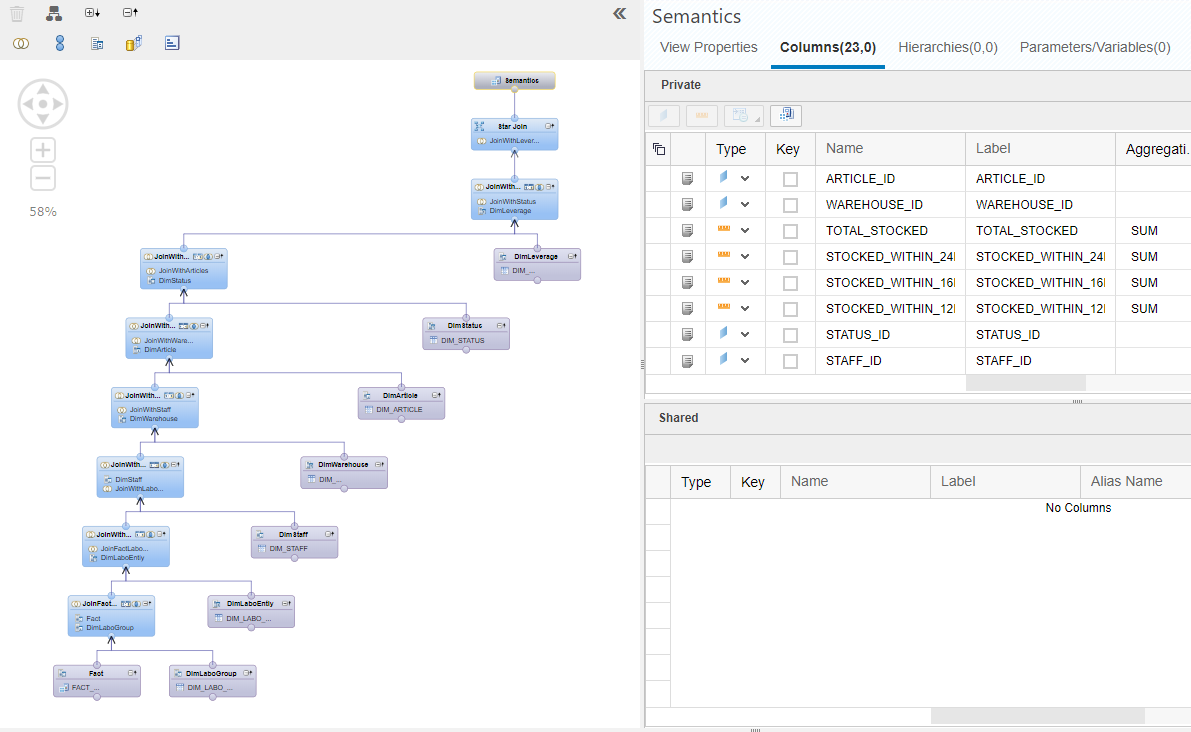
\includegraphics[scale=0.5]{../images/DM_FG_datamart.png}
	\caption{Sterschema opgesteld in SAP voor het dimensioneel model.}
	\label{fig:dmdmart}
\end{figure}


